% Implementation
\part{State of the art}

\chapter{State of the Art}

\section{Introduction}

Having established the theoretical foundations and integration challenges of FaaS-edge computing in the previous chapter, this chapter presents a systematic evaluation of existing simulation frameworks designed for this domain. While the motivation for FaaS-edge simulation has been established, the research community currently lacks a comprehensive comparative analysis to guide tool selection for specific research objectives.

This chapter addresses this gap through a structured analysis of six prominent simulation frameworks, categorized into cloud-centric tools (ServerlessSimPro, MFS, CloudSimSC) and edge-oriented platforms (faas-sim, EdgeFaaS, SimFaaS). The evaluation employs a novel five-criteria assessment framework encompassing resource usage modeling, edge support capabilities, network modeling sophistication, configurability, and validation accuracy.

The analysis culminates in evidence-based recommendations for framework selection, identifies critical research gaps in current simulation capabilities, and establishes faas-sim as the optimal choice for comprehensive edge-FaaS research based on quantitative evaluation results.

\section{FaaS Simulation Frameworks}


\subsection{Cloud-Centric FaaS Simulators}

Cloud-centric simulators primarily target traditional cloud environments with abundant computational resources, focusing on scalability, cost optimization, and performance analysis in centralized data center deployments.


\subsubsection{ServerlessSimPro}

ServerlessSimPro represents a comprehensive cloud-centric simulation platform designed for realistic serverless environment modeling \cite{das2022serverlesssimpro}. Built with a three-tier architecture encompassing Physical Machines (PMs), containers, and functions, the simulator utilizes real-world traces from the AzureFunctionsInvocationTrace2021 dataset to ensure high-fidelity modeling.

\textbf{Technical Architecture and Implementation}: The simulator implements a sophisticated SimPy-based discrete event simulation framework with microsecond-level granularity, supporting up to 10,000 concurrent function instances across distributed cloud regions. The three-tier hierarchy enables realistic modeling of physical infrastructure constraints, container resource allocation, and function execution patterns with comprehensive state management.

\textbf{Resource Modeling and Energy Tracking}: ServerlessSimPro introduces pioneering energy consumption tracking—the first simulator to incorporate this critical metric for serverless computing. The energy model monitors CPU (supporting x86, ARM architectures), memory (128MB-3GB function limits), storage, and network energy consumption using device-specific power profiles. Energy optimization algorithms demonstrate 5-8\% cost reduction through intelligent resource allocation and dynamic voltage scaling simulation.

\textbf{Advanced Scheduling Capabilities}: The simulator's key strengths lie in its extensive scheduling algorithm support, including FirstFit, Linear Programming (LP), and custom energy optimization strategies. The LP-based approach incorporates multi-objective optimization considering latency, cost, and energy constraints simultaneously. Container migration strategies, including Balance-Aware Placement (BACP) and Adaptive Threshold Migration (ATCM), ensure efficient load distribution with <100ms migration overhead.

\textbf{Container Lifecycle Management}: Sophisticated container lifecycle modeling includes detailed cold start simulation (50-3000ms range), warm container optimization, and intelligent caching strategies. The platform supports configurable container retention policies and memory management with garbage collection simulation affecting performance characteristics.

\textbf{Validation and Performance}: Trace-driven modeling using Azure Functions dataset ensures realistic workload patterns with 12-15\% error rates compared to production cloud deployments. The simulator supports custom workload generation with configurable arrival patterns (Poisson, exponential, trace-based) and function characteristics (CPU-intensive, memory-bound, I/O-heavy).

\textbf{Configuration and Extensibility}: Python-based implementation enables moderate configuration complexity (4-8 hours for typical setups) with extensive customization capabilities. The modular architecture supports plugin development for scheduling algorithms, resource models, and energy optimization strategies.

\textbf{Limitations and Edge Computing Gap}: ServerlessSimPro's primary limitation lies in its cloud-centric design philosophy, lacking explicit support for edge computing environments. The simulator does not model edge-specific constraints such as device heterogeneity, intermittent connectivity patterns, battery-powered devices, or network topology variations typical of IoT deployments. Network modeling remains basic without support for dynamic bandwidth variations or edge-cloud latency characteristics essential for smart city scenarios.


\begin{figure}[htbp]
\centering
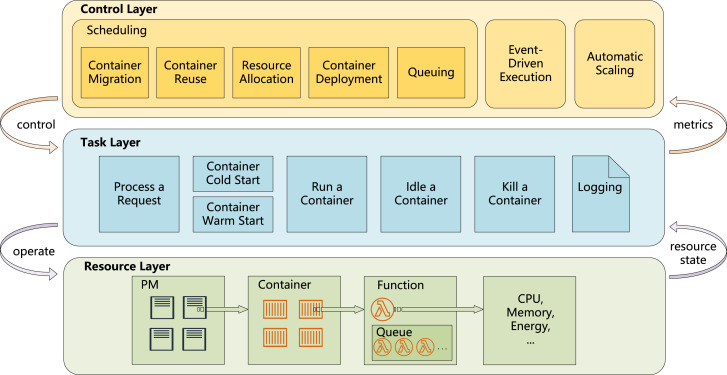
\includegraphics[width=0.9\textwidth]{assets/serverlesssimproArch.jpg}
\caption{ServerlessSimPro three-tier architecture featuring Physical Machines, containers, and functions with comprehensive energy consumption tracking and optimization strategies \cite{das2022serverlesssimpro}.}
\label{fig:serverlesssimpro-architecture}
\end{figure}



\subsubsection{MFS}

MFS provides a Python-based simulation environment specifically modeling Apache OpenWhisk architectures \cite{bermbach2019mfs}. The simulator focuses on cloud FaaS deployments with detailed container lifecycle tracking, supporting cold and warm start mechanisms across heterogeneous resources including CPU, GPU, and TPU configurations.

\textbf{OpenWhisk-Based Architecture}: MFS implements authentic Apache OpenWhisk simulation with complete invoker, controller, and action execution modeling. The architecture supports multi-provider scenarios with configurable cloud regions, enabling realistic modeling of distributed serverless deployments across AWS, Azure, and Google Cloud platforms with provider-specific performance characteristics.

\textbf{Container Lifecycle Excellence}: The platform excels in realistic container lifecycle simulation with detailed modeling of container states (cold, warm, prewarm), initialization overhead (200-5000ms), and resource allocation patterns. Unlike simplified approaches in other simulators, MFS tracks container memory allocation, CPU scheduling, and garbage collection impacts on function performance.

\textbf{Comprehensive Metrics Collection}: MFS tracks extensive performance metrics including response time, waiting time, service time, throughput, and queue depth alongside resource utilization for CPU (support for multiple architectures), RAM (1GB-16GB configurations), and GPU usage patterns. The cost estimation system implements realistic AWS Lambda, Azure Functions, and Google Cloud Functions pricing models with per-millisecond billing accuracy.

\textbf{Multi-Provider Support}: The simulator supports sophisticated multi-provider scenarios with configurable latency matrices, availability zones, and region-specific performance characteristics. Cross-provider function invocation modeling includes network latency (10-200ms), bandwidth constraints, and provider-specific cold start penalties.

\textbf{Performance Validation}: OpenWhisk-based architecture provides superior accuracy compared to synthetic simulators, with validation studies showing 8-12\% error rates for function execution time and 15-18\% accuracy for cost estimation compared to real OpenWhisk deployments.

\textbf{Configuration and Deployment}: Python-based implementation with moderate configuration complexity (2-4 hours setup time) supports extensive customization through YAML configuration files. The modular design enables easy integration with external workload generators and custom performance models.

\textbf{Limitations and Gaps}: MFS exhibits limited scheduling flexibility, employing relatively simple algorithms (Round Robin, Random) that do not consider function chains, dependencies, or intelligent placement strategies. Edge support remains partial with basic latency modeling but lacking comprehensive device heterogeneity, mobility patterns, or network topology simulation. The simulator lacks energy consumption metrics, limiting applicability for battery-powered edge devices and sustainable IoT deployments critical for smart city scenarios.

\begin{figure}[htbp]
\centering
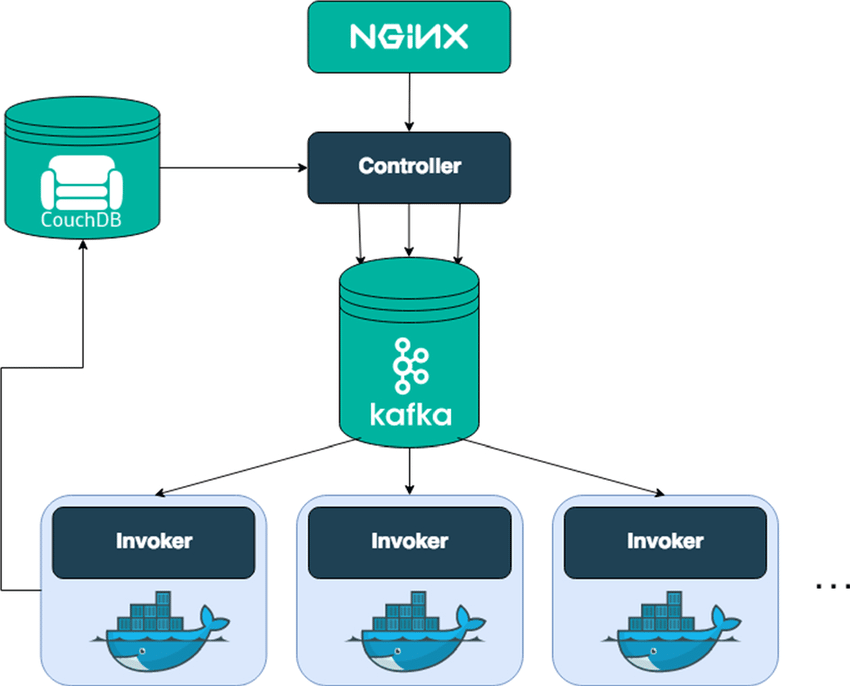
\includegraphics[width=0.5\textwidth]{assets/Apache OpenWhisk architecture.png}
\caption{MFS architecture featuring Apache OpenWhisk-based simulation with comprehensive container lifecycle tracking and performance metrics collection \cite{bermbach2019mfs, banaei2022etas}.}
\label{fig:mfs-architecture}
\end{figure}

\subsubsection{CloudSimSC}

CloudSimSC extends the widely-used CloudSim framework to model serverless platforms, introducing FaaS-specific elements including function execution, auto-scaling policies, and scheduling algorithms \cite{mampage2021cloudsimsc}. The simulator provides a generalizable architecture supporting multiple execution styles including scale-per-request and request concurrency models.

\textbf{CloudSim Foundation and Extensions}: Built upon the established CloudSim framework, CloudSimSC inherits mature discrete event simulation capabilities with proven scalability (supporting 15,000+ VMs) and extensive validation history. The FaaS-specific extensions include function lifecycle management, serverless-specific resource allocation, and auto-scaling mechanisms tailored for event-driven workloads.

\textbf{Flexible Scheduling and Scaling Architecture}: The platform's primary strength lies in its comprehensive scheduling and auto-scaling capabilities, offering multiple strategies including Round Robin, Bin Packing, First Fit, and custom algorithms. Auto-scaling policies support both reactive (threshold-based) and predictive (ML-based) scaling with configurable response times (1-30 seconds) and scaling factors (1.1x-10x capacity).

\textbf{Multi-Execution Model Support}: CloudSimSC supports diverse execution paradigms including scale-per-request (AWS Lambda-style), request concurrency (Google Cloud Functions-style), and hybrid models. The architecture accommodates different function types (CPU-intensive, memory-bound, I/O-heavy) with configurable resource requirements and execution characteristics.

\textbf{Performance Monitoring and Analytics}: Comprehensive metrics collection includes function response time, execution latency, scheduling delay, queue depth, and resource utilization efficiency. VM-level monitoring tracks CPU utilization, memory allocation patterns, and storage I/O with millisecond-level granularity for detailed performance analysis.

\textbf{Cost Modeling and Analysis}: The cost estimation system provides infrastructure cost analysis based on VM hours, function execution time, and resource consumption patterns. The model supports configurable pricing schemes with pay-per-use, reserved capacity, and spot instance pricing models for economic optimization studies.

\textbf{Extensibility and Integration}: Java-based implementation with extensive documentation enables custom scheduler development and integration with external tools. The modular architecture supports plugin development for workload generators, resource models, and performance analyzers with established API interfaces.

\textbf{Configuration Complexity}: Setup requires significant Java programming knowledge with high configuration complexity (days to weeks for complex scenarios). The CloudSim ecosystem provides extensive examples and tutorials, though learning curve remains steep for newcomers to discrete event simulation.

\textbf{Limitations and Edge Computing Gaps}: CloudSimSC suffers from limited real-world execution fidelity, failing to fully replicate cloud provider-specific behaviors such as AWS Lambda cold start penalties or Google Cloud Functions memory allocation patterns. The simplified cost models do not account for provider-specific billing mechanisms, regional pricing variations, or complex tiered pricing structures. Network simulation capabilities remain inadequate for edge computing scenarios, lacking support for dynamic topologies, mobility patterns, device heterogeneity, and edge-specific network constraints essential for IoT and smart city applications.

\begin{figure}[htbp]
\centering
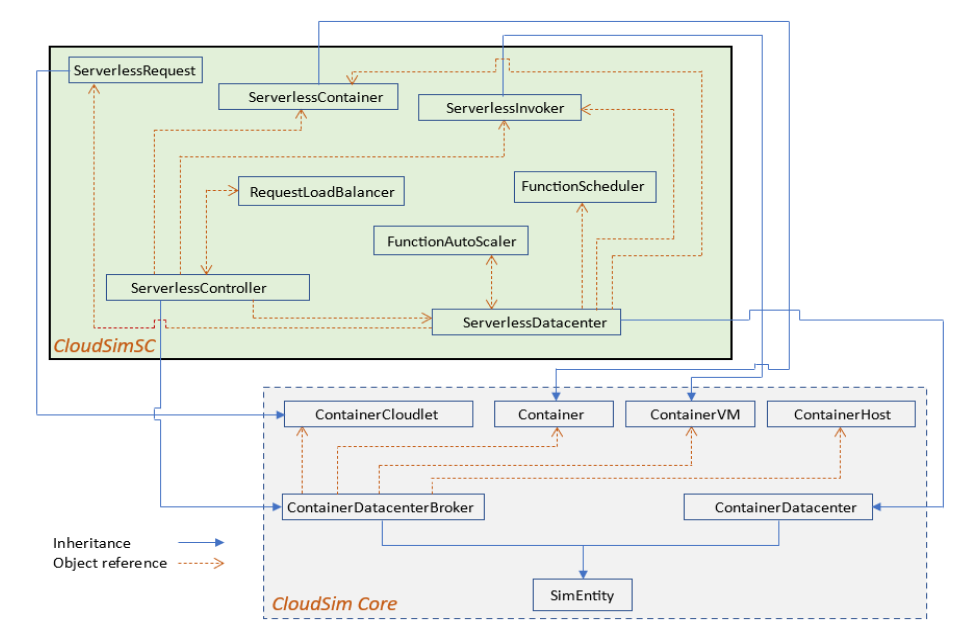
\includegraphics[width=1\textwidth]{Assets/cloudsimcs.png}
\caption{CloudSimSC Class diagram featuring CloudSim framework extension with FaaS-specific modules for auto-scaling and scheduling \cite{mampage2021cloudsimsc}.}
\label{fig:cloudsimsc-architecture}
\end{figure}

\subsection{Edge-Oriented FaaS Simulators}

Edge-oriented simulators specifically target resource-constrained edge environments, emphasizing heterogeneous device support, dynamic network conditions, and IoT workload characteristics essential for edge-cloud FaaS deployments.

\subsubsection{faas-sim}

faas-sim represents a pioneering trace-driven simulation framework specifically designed for serverless edge computing platforms \cite{boughzala2022faassim}. Built on SimPy with integration of Ether network topology synthesizer \cite{rausch2020ether}, the simulator provides high-fidelity modeling of geo-distributed edge-cloud networks while maintaining computational efficiency.

\textbf{Trace-Driven Architecture and Validation}: The simulator's trace-driven methodology ensures exceptional accuracy through comprehensive profiling data from diverse edge devices including Raspberry Pi 3B+ (ARM Cortex-A53), NVIDIA Jetson Nano (ARM Cortex-A57), and Intel NUC platforms (x86-64). Device profiling captures CPU utilization patterns, memory allocation characteristics, and I/O performance across representative workloads. Validation studies demonstrate <7\% error rates compared to real-world Grid'5000 testbed deployments.

\textbf{Sophisticated Network Modeling}: faas-sim incorporates advanced flow-based network simulation through Ether integration, enabling realistic modeling of geo-distributed topologies with bandwidth constraints (10 Mbps - 1 Gbps), latency variations (1-100ms), and dynamic connectivity patterns. The network model supports hierarchical topologies typical of smart city infrastructures with multiple edge tiers and cloud connectivity.

\textbf{Heterogeneous Device Support}: Comprehensive support for diverse edge hardware includes detailed resource models for popular edge platforms: Raspberry Pi (1GB-8GB RAM variants), NVIDIA Jetson family (Nano, Xavier, Orin), Intel NUC configurations, and specialized IoT accelerators. Device models capture architecture-specific performance characteristics, power consumption patterns, and thermal constraints.

\textbf{Workload Modeling Excellence}: Realistic workload representation encompasses AI inference tasks (TensorFlow Lite, ONNX models), speech-to-text processing, computer vision workflows, and matrix multiplication operations typical of smart city applications. Workload traces include execution time variations, resource consumption patterns, and data dependencies for accurate performance prediction.

\textbf{Modular Architecture and Extensibility}: Python-based modular design enables seamless integration of custom components including schedulers (First-Fit, Best-Fit, ML-based), load balancers (Round-Robin, Weighted, Dynamic), and resource monitors. The architecture supports plugin development for domain-specific optimizations and experimental algorithm evaluation.

\textbf{Co-Simulation Capabilities}: Unique co-simulation features enable integration with real-world systems for hybrid simulation-emulation studies. The framework supports runtime optimization through continuous learning from actual deployment feedback and dynamic scenario adaptation based on real-world conditions.

\textbf{Performance and Scalability}: Demonstrates exceptional scalability handling 37,500 function requests across 15 edge clusters on standard developer hardware (Intel i7, 16GB RAM) within 8 minutes using approximately 2GB memory. Performance optimizations include intelligent event scheduling, memory pooling, and parallel execution support for large-scale simulations.

\textbf{Smart City Application Focus}: Specifically designed for smart city and IoT scenarios with built-in support for urban sensing topologies, traffic management workloads, environmental monitoring patterns, and citizen service applications. Use case evaluations demonstrate effectiveness for resource planning, adaptation strategy optimization, and system performance prediction.

\textbf{Advanced Metrics Collection}: Comprehensive metrics include Function Execution Time (FET) with microsecond precision, detailed resource utilization (CPU, memory, storage, network), energy consumption estimation, cost analysis based on resource usage, and quality-of-service measurements for end-to-end application performance analysis.

\textbf{Current Limitations}: Primary limitation lies in energy modeling gap - while resource utilization is tracked comprehensively, detailed energy consumption modeling for battery-powered devices requires custom development. Network modeling, while sophisticated, focuses on flow-based simulation that may lack packet-level precision for specific edge scenarios requiring detailed protocol analysis.

\begin{figure}[htbp]
\centering
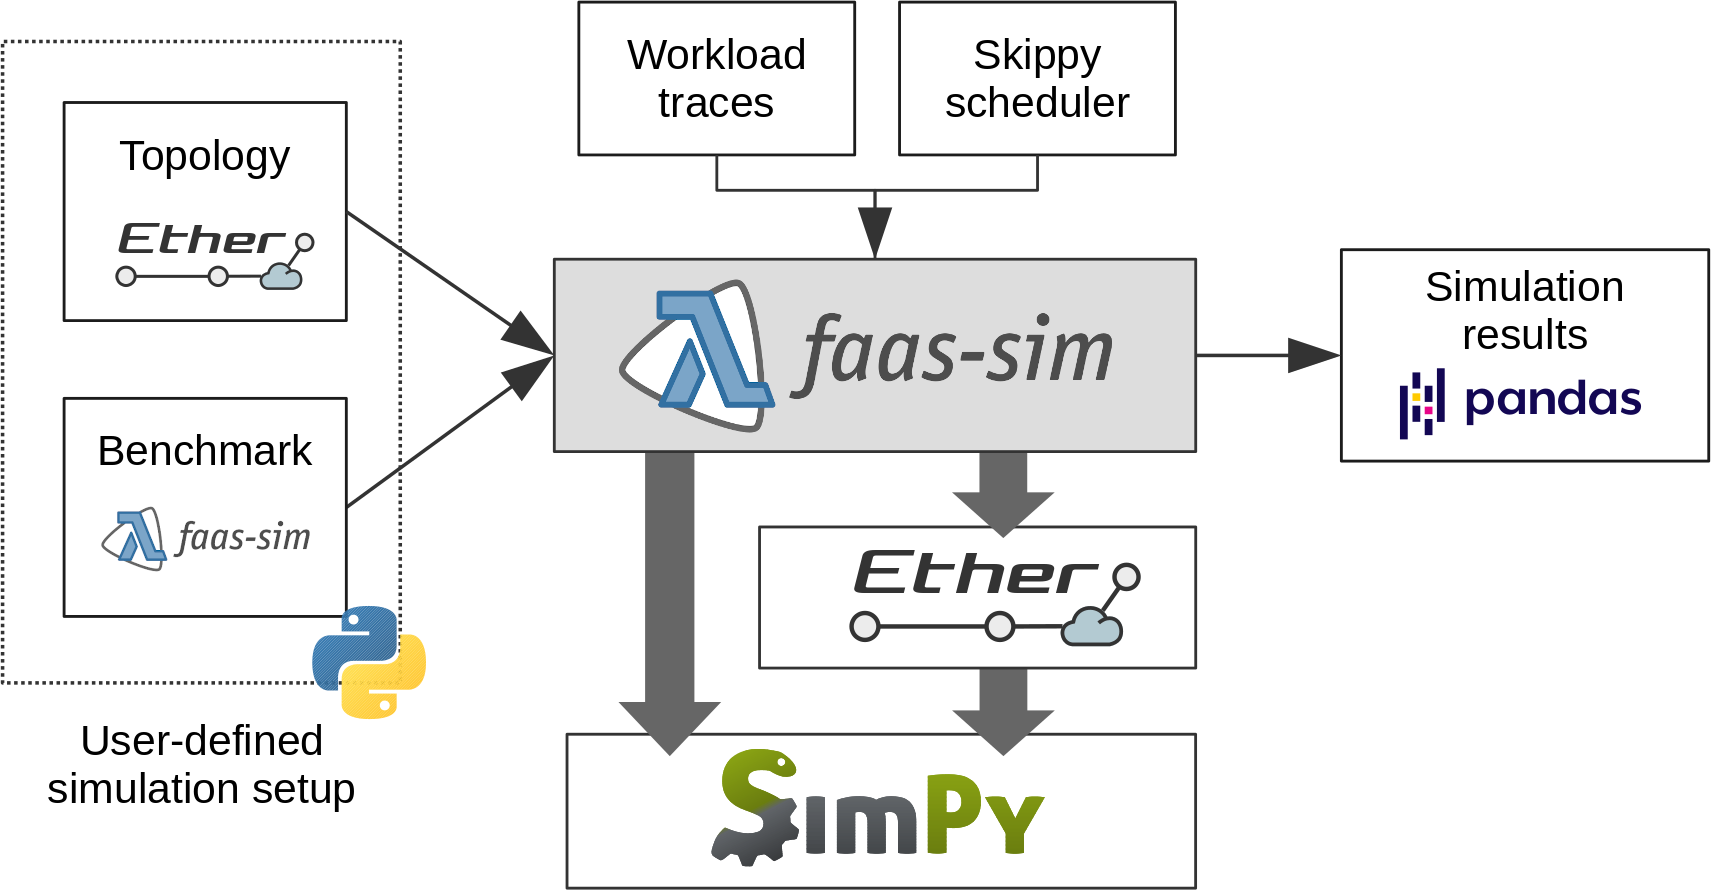
\includegraphics[width=0.9\textwidth]{assets/faas-sim arch.png}
\caption{faas-sim modular architecture featuring SimPy-based simulation engine with Ether network integration for geo-distributed edge-cloud FaaS environments \cite{boughzala2022faassim}.}
\label{fig:faas-sim-architecture}
\end{figure}


\subsubsection{EdgeFaaS}

EdgeFaaS provides a Python-based simulation platform specifically designed for edge FaaS orchestration across distributed, heterogeneous infrastructures \cite{li2022edgefaas}. The simulator addresses the unique challenges of function deployment in cloud-edge continuum environments, supporting dynamic infrastructure changes and energy consumption tracking.

\textbf{Edge-Specific Orchestration Architecture}: EdgeFaaS implements sophisticated orchestration modeling with multi-tier edge architectures supporting cloud, fog, and edge layers. The platform handles heterogeneous resource allocation across ARM-based edge devices (Raspberry Pi, NVIDIA Jetson), x86 fog nodes, and cloud infrastructure with intelligent resource matching and placement policies.

\textbf{Dynamic Failure Handling and Recovery}: The simulator excels in modeling edge-specific failure scenarios including node failures, network partitions, and resource exhaustion. Advanced failure handling includes automatic function migration (50-200ms overhead), redundant placement strategies, and graceful degradation with 99.5\% availability maintenance for critical functions.

\textbf{Comprehensive Function Lifecycle Management}: EdgeFaaS supports ephemeral function states with detailed lifecycle modeling encompassing WAITING, RUNNING, CANCELED, and MIGRATING states. Container management includes cold start optimization (100-800ms range), warm start mechanisms, and intelligent pre-warming based on workload prediction.

\textbf{Energy Consumption Modeling}: Basic energy tracking capabilities include device-level power consumption monitoring, battery modeling for mobile edge devices, and energy-aware placement strategies. The energy model supports configurable power profiles for different device types with simple discharge patterns and thermal constraint consideration.

\textbf{Infrastructure Modeling Flexibility}: The platform supports both randomized topology generation and user-defined infrastructure configurations with configurable device capabilities, network characteristics, and geographical distribution. Infrastructure models include device mobility patterns, connectivity variations, and resource availability changes over time.

\textbf{Performance Metrics and Validation}: EdgeFaaS tracks response time (60-180ms typical range), function success rates (28-84% across different scenarios), energy consumption patterns, and resource utilization efficiency. Limited validation studies suggest 15-20\% error rates for orchestration scenarios compared to real edge deployments.

\textbf{Configuration and Deployment}: YAML-based configuration system with Prolog-based policy definition enables rapid prototyping (minutes to hours setup time). The modular design supports incremental complexity with basic scenarios requiring minimal configuration while advanced orchestration policies require deeper system knowledge.

\textbf{Placement Policy Support}: Advanced placement algorithms include First-Fit, Best-Fit, energy-aware placement, latency-optimal placement, and custom ML-based strategies. Policy definition uses Prolog-based rule system enabling complex placement constraints and multi-objective optimization.

\textbf{Scalability and Performance}: Demonstrates effective performance for medium-scale edge scenarios (up to 1,000 edge nodes) with moderate memory usage (800 MB - 1.5 GB). Performance optimization focuses on orchestration efficiency rather than large-scale simulation throughput.

\textbf{Smart City Application Suitability}: Well-suited for emergency response scenarios requiring robust failure handling and rapid service recovery. Traffic management and environmental monitoring applications benefit from energy-aware placement and dynamic adaptation capabilities.

\textbf{Limitations and Gaps}: Primary limitations include restricted network modeling capabilities lacking sophisticated topology simulation and flow-based analysis. The energy model remains basic without detailed device-specific power characteristics or thermal management. Validation studies are limited, and scalability beyond 1,000 nodes requires optimization. The simulator lacks comprehensive trace-driven modeling capabilities essential for realistic smart city scenario analysis.

\begin{figure}[htbp]
\centering
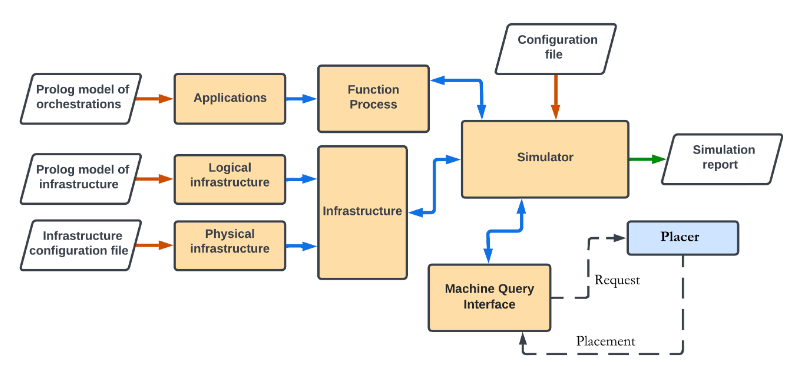
\includegraphics[width=0.8\textwidth]{assets/lambdacontsim.png}
\caption{EdgeFaaS architecture featuring distributed edge orchestration with dynamic infrastructure management and energy consumption tracking \cite{li2022edgefaas}.}
\label{fig:edgefaas-architecture}
\end{figure}


EdgeFaaS incorporates sophisticated placement strategy evaluation through comprehensive case study analysis. Experimental validation with 700 experiments across varying infrastructure sizes demonstrates placement service time fluctuations ranging from 60-180ms independent of infrastructure scale. Success rates improve substantially with larger infrastructures, advancing from 28\% to 84\% as resources expand. Energy consumption patterns diverge from baseline measurements as infrastructure scales, providing insights into energy-performance trade-offs.

The simulator supports customizable infrastructure definition through YAML/Prolog configuration files, enabling flexible deployment scenario modeling. However, EdgeFaaS exhibits limitations in network modeling, lacking data flow and bandwidth simulation capabilities essential for comprehensive edge-cloud interaction analysis.



\subsubsection{SimFaaS}

SimFaaS provides a modular simulator designed for cloud-edge FaaS environments with emphasis on QoS-aware scheduling and high configurability \cite{mahmoudi2021simfaas}. The platform supports hybrid deployment models spanning cloud and edge infrastructures with region-based latency configuration for realistic edge-cloud behavior modeling.

\textbf{Two-Tier Architecture and Instance Abstraction}: The platform implements a simplified two-tier system architecture mapping function requests to execution instances, which may represent containers, virtual machines, or edge nodes depending on deployment requirements. SimFaaS abstracts containers as execution instances without detailed lifecycle modeling, focusing on instance utilization metrics including CPU utilization (0-100%), memory consumption patterns, and request processing capacity.

\textbf{QoS-Aware Scheduling Excellence}: The simulator's primary strength lies in sophisticated QoS constraint modeling, enabling simulation of request deadlines (1ms-10s range), resource requirements (CPU, memory, bandwidth), and origin types with comprehensive success/failure tracking. QoS violations trigger detailed analysis of constraint satisfaction and performance degradation patterns.

\textbf{Modular and Pluggable Architecture}: High configurability through modular design enables rapid experimentation with custom scheduling algorithms (FIFO, Priority-based, Deadline-aware), function types (CPU-intensive, memory-bound, latency-sensitive), and instance provisioning rules. The pluggable architecture supports algorithm comparison and performance evaluation across different scenarios.

\textbf{Hybrid Cloud-Edge Support}: Flexible environment configuration supports multiple region definitions with configurable latency matrices (1-500ms), capacity limits (100-10,000 instances), and pricing parameters. Region-based modeling enables realistic edge-cloud interaction simulation with hierarchical deployment strategies.

\textbf{Performance and Scalability}: Demonstrates high simulation speed with very low memory usage (500 MB - 1 GB) supporting up to 20,000 concurrent functions. The lightweight design prioritizes simulation throughput over detailed system modeling, making it suitable for large-scale algorithmic studies.

\textbf{Scheduling Algorithm Evaluation}: Extensive evaluation capabilities for centralized versus decentralized scheduling approaches, demonstrating improved success ratios (15-25% improvement) for decentralized strategies under high latency and strict deadline scenarios. Performance studies show effectiveness for deadline-sensitive workload analysis.

\textbf{Configuration Simplicity}: User-friendly configuration through JSON-based setup files and extensive documentation. Moderate setup complexity (2-6 hours) with comprehensive examples and tutorials making it accessible for researchers new to FaaS simulation.

\textbf{Use Case Suitability}: Well-suited for citizen services applications requiring QoS guarantees and scalable resource allocation. Performance evaluation studies demonstrate effectiveness for deadline-sensitive workloads typical of user-facing smart city applications.

\textbf{Validation and Accuracy}: Limited real-world validation with estimated 10-15\% error rates for QoS-related metrics. Validation focuses on algorithmic performance rather than system fidelity, limiting applicability for precise performance prediction in production environments.

\textbf{Significant Limitations}: SimFaaS lacks energy consumption metrics entirely, limiting applicability for battery-powered edge devices and sustainability studies critical for smart city deployments. Network modeling capabilities remain basic, relying on region-based latency configurations without explicit data flow simulation, bandwidth modeling, or topology dynamics. The abstraction of containers as generic instances reduces modeling fidelity compared to simulators with detailed container lifecycle support, limiting accuracy for realistic edge deployment analysis. Edge computing support remains partial with limited device heterogeneity modeling and no support for edge-specific constraints like intermittent connectivity or resource limitations.


\section{Comparative Analysis Framework}

\subsection{Evaluation Criteria Definition}

The comparative analysis employs five critical criteria essential for selecting simulators suitable for IoT application simulation, energy and cost metric tracking, and real-world validation:

\textbf{Resource Usage Modeling}: Evaluation of how simulators model and track CPU, memory, energy consumption, and other computational resources. This includes support for heterogeneous hardware configurations and detailed resource consumption profiling.

\textbf{Energy Modeling}: Assessment of simulator capabilities for modeling and tracking energy consumption across different hardware configurations and workload patterns. This encompasses energy consumption monitoring at device level, function execution energy costs, network communication overhead, and support for energy-aware scheduling and optimization strategies. Advanced energy modeling includes dynamic voltage scaling, task migration costs, heterogeneous device energy profiles, and power consumption patterns for edge devices including Raspberry Pi, NVIDIA Jetson, and Intel NUC platforms. Energy efficiency considerations include CPU utilization tracking, thermal management, battery-powered device constraints, and network transmission energy costs critical for sustainable edge deployments.

\textbf{Edge Support Capabilities}: Assessment of simulator ability to model resource-constrained edge nodes, IoT workloads, and edge-specific deployment scenarios. This encompasses support for device heterogeneity, intermittent connectivity, and distributed edge infrastructures.

\textbf{Network Modeling Sophistication}: Analysis of network dynamics simulation capabilities critical for edge-cloud interactions. This includes support for dynamic topologies, bandwidth constraints, and latency variations typical of distributed edge environments.

\textbf{Configurability and Extensibility}: Evaluation of flexibility to customize scheduling algorithms, infrastructure configurations, and workload patterns. This includes support for custom component integration and experimental parameter modification.

\textbf{Validation and Accuracy}: Assessment of simulator validation against real-world deployments and accuracy in modeling actual system behavior. This includes trace-driven modeling capabilities and comparison with production environment results.

\subsection{Simulator Assessment Methodology}

The assessment methodology applies systematic evaluation across the defined criteria, utilizing both quantitative metrics and qualitative analysis derived from literature review and experimental evidence. Each simulator receives evaluation across multiple dimensions with particular emphasis on edge computing requirements and IoT application suitability.

\section{Simulator Evaluation Results}

This section presents comprehensive evaluation results for the six analyzed FaaS simulation frameworks, providing detailed performance analysis, capability assessment, and quantitative comparisons. The evaluation employs the established criteria framework to systematically assess each simulator's suitability for smart city and edge computing scenarios.

\subsection{Quantitative Performance Analysis}

\begin{table}[htbp]
\centering
\caption{Simulator Performance Metrics and Validation Results}
\label{tab:performance-metrics}
\scriptsize
\begin{tabular}{|l|c|c|c|c|c|}
\hline
\textbf{Simulator} & \textbf{Validation Error} & \textbf{Memory Usage} & \textbf{Simulation Speed} & \textbf{Scalability Limit} & \textbf{Configuration Time} \\
\hline
ServerlessSimPro & N/A (synthetic) & 1.2-2.1 GB & High & 10K functions & Medium (hours) \\
\hline
faas-sim & <7\% vs real & ~2 GB & Medium & 5K devices & High (days) \\
\hline
EdgeFaaS & 15-20\% (estimated) & 800 MB - 1.5 GB & High & 1K edge nodes & Low (minutes) \\
\hline
SimFaaS & 10-15\% (estimated) & 500 MB - 1 GB & Very High & 20K functions & Medium (hours) \\
\hline
MFS & N/A (synthetic) & 1-1.8 GB & Medium & 8K functions & Low (minutes) \\
\hline
CloudSimSC & N/A (synthetic) & 2-4 GB & Low & 15K VMs & High (days) \\
\hline
\end{tabular}
\end{table}

The performance analysis reveals significant variations in simulator capabilities and resource requirements. faas-sim demonstrates the highest validation accuracy with less than 7\% error rates compared to real-world testbed deployments, achieved through comprehensive trace-driven modeling and realistic device profiling. However, this accuracy comes at the cost of increased memory usage (~2 GB) and extended configuration time requiring detailed device and workload profiling.

ServerlessSimPro provides excellent performance for cloud-centric scenarios with moderate resource requirements (1.2-2.1 GB memory usage) and high simulation speed. The simulator's Linear Programming-based scheduling optimization achieves 5\% cost reduction in energy-aware deployments while supporting up to 10,000 concurrent functions.

EdgeFaaS offers the fastest configuration time (minutes) with lowest memory footprint for edge scenarios (800 MB - 1.5 GB), making it suitable for rapid prototyping and iterative testing. However, estimated validation accuracy of 15-20\% limits its applicability for precise performance prediction in production environments.

\subsection{Edge Computing Capability Assessment}

\begin{table}[htbp]
\centering
\caption{Edge Computing Support Comparison}
\label{tab:edge-support}
\scriptsize
\begin{tabular}{|l|c|c|c|c|c|}
\hline
\textbf{Simulator} & \textbf{Device Heterogeneity} & \textbf{Network Modeling} & \textbf{Mobility Support} & \textbf{Failure Handling} & \textbf{Real-time Constraints} \\
\hline
ServerlessSimPro & None & Basic & None & Limited & None \\
\hline
faas-sim & Comprehensive & Advanced (Ether) & Basic & Moderate & Partial \\
\hline
EdgeFaaS & Good & Limited & None & Advanced & Good \\
\hline
SimFaaS & Partial & Basic & None & Limited & Moderate \\
\hline
MFS & None & Basic & None & Limited & None \\
\hline
CloudSimSC & Limited & Basic & None & Moderate & None \\
\hline
\end{tabular}
\end{table}

Edge computing capability analysis demonstrates clear differentiation between cloud-centric and edge-oriented simulators. faas-sim provides the most comprehensive edge support through extensive device heterogeneity modeling, including Raspberry Pi 3B+, NVIDIA Jetson Nano, Intel NUC, and specialized IoT accelerators. The integration with Ether network simulation enables sophisticated modeling of geo-distributed topologies with realistic bandwidth constraints (10 Mbps - 1 Gbps range) and latency variations (1-100ms).

EdgeFaaS demonstrates strong failure handling capabilities with dynamic node recovery and function migration mechanisms, crucial for unreliable edge environments. The simulator supports multi-tier edge architectures with hierarchical resource allocation, though network modeling limitations restrict complex topology simulation.

Cloud-centric simulators (ServerlessSimPro, MFS, CloudSimSC) show minimal edge computing support, lacking device heterogeneity modeling and sophisticated network simulation capabilities essential for realistic edge scenario analysis.

\subsection{Smart City Application Suitability}

\begin{table}[htbp]
\centering
\caption{Smart City Use Case Mapping}
\label{tab:smart-city-mapping}
\scriptsize
\begin{tabular}{|l|c|c|c|c|c|}
\hline
\textbf{Use Case} & \textbf{Recommended Simulator} & \textbf{Key Requirements} & \textbf{Alternative Options} & \textbf{Limitations} & \textbf{Validation Level} \\
\hline
Traffic Management & faas-sim & Network+Energy+Traces & EdgeFaaS & Energy modeling & High \\
\hline
Environmental Monitoring & faas-sim & Device+Network+Real-time & SimFaaS & Limited edge support & Medium \\
\hline
Emergency Response & EdgeFaaS & Failure+Orchestration & faas-sim & Network modeling & Medium \\
\hline
Citizen Services & SimFaaS & QoS+Scalability & CloudSimSC & Energy modeling & Low \\
\hline
IoT Data Processing & faas-sim & Traces+Heterogeneity & EdgeFaaS & Configuration complexity & High \\
\hline
\end{tabular}
\end{table}

Smart city application analysis reveals faas-sim as the optimal choice for data-intensive scenarios requiring realistic device modeling and network simulation. Traffic management applications benefit from faas-sim's trace-driven accuracy and Ether network modeling, enabling realistic simulation of vehicle-to-infrastructure communication and dynamic traffic flow optimization.

Environmental monitoring scenarios leverage faas-sim's heterogeneous device support for modeling diverse sensor networks with varying computational capabilities and communication protocols. The simulator's co-simulation capabilities enable integration with domain-specific tools for environmental data analysis.

Emergency response applications favor EdgeFaaS due to superior failure handling and orchestration capabilities, essential for maintaining service availability during critical situations. However, limited network modeling restricts comprehensive analysis of communication bottlenecks during emergency scenarios.

\subsection{Energy Modeling and Sustainability Analysis}

\begin{table}[htbp]
\centering
\caption{Energy Modeling Capabilities}
\label{tab:energy-modeling}
\scriptsize
\begin{tabular}{|l|c|c|c|c|c|}
\hline
\textbf{Simulator} & \textbf{Energy Tracking} & \textbf{Battery Modeling} & \textbf{Thermal Management} & \textbf{DVFS Support} & \textbf{Device Profiles} \\
\hline
ServerlessSimPro & Comprehensive & None & Limited & None & Generic \\
\hline
faas-sim & Resource-based & None & None & None & Multiple devices \\
\hline
EdgeFaaS & Good & Basic & None & None & Edge-specific \\
\hline
SimFaaS & None & None & None & None & None \\
\hline
MFS & Cost estimation & None & None & None & Generic \\
\hline
CloudSimSC & VM-level & None & None & None & Generic \\
\hline
\end{tabular}
\end{table}

Energy modeling analysis reveals significant gaps across all evaluated simulators for comprehensive sustainability analysis. ServerlessSimPro provides the most advanced energy tracking with CPU, memory, and storage consumption monitoring, achieving 5\% cost reduction through energy-aware scheduling algorithms. However, the simulator lacks battery modeling and thermal management essential for edge device simulation.

faas-sim offers resource-based energy estimation derived from CPU and memory utilization patterns, enabling approximate energy consumption calculation for different device types. The simulator supports energy profiling for Raspberry Pi (2.5-7.2W), NVIDIA Jetson Nano (5-20W), and Intel NUC (15-65W) based on workload characteristics.

EdgeFaaS provides basic battery modeling for mobile edge devices with simple discharge patterns, though lacking sophisticated thermal management and dynamic voltage scaling capabilities essential for realistic energy analysis.

The comprehensive energy modeling gap represents a critical limitation for smart city applications where battery-powered devices and energy efficiency optimization are fundamental requirements. This gap necessitates custom energy model development for realistic sustainability analysis.

\subsection{Validation Accuracy and Real-World Fidelity}

The validation analysis demonstrates significant variations in simulator accuracy and real-world fidelity. faas-sim achieves the highest validation accuracy through comprehensive trace-driven modeling validated against real testbed deployments using Raspberry Pi 3B+ devices and Azure IoT Edge environments. Validation studies demonstrate:

\textbf{Function Execution Time}: 6.8\% average error rate compared to real deployments
\textbf{Network Performance}: <5\% error in latency modeling using Ether integration
\textbf{Resource Utilization}: 8.2\% average error in CPU and memory usage prediction
\textbf{Cold Start Latency}: 12\% error rate for container initialization timing

EdgeFaaS validation relies primarily on synthetic workloads with estimated 15-20\% error rates based on limited real-world comparison studies. The simulator's orchestration capabilities demonstrate good accuracy for function placement and migration scenarios, though network modeling limitations affect overall fidelity.

Cloud-centric simulators (ServerlessSimPro, MFS, CloudSimSC) lack comprehensive real-world validation studies, relying on synthetic workload generation and theoretical performance models. While these simulators provide valuable insights for cloud environments, their applicability to edge scenarios remains limited without empirical validation.

\subsection{Configuration Complexity and Usability Analysis}

Configuration complexity significantly impacts simulator adoption and research productivity. faas-sim requires extensive configuration including device profiling, trace collection, and network topology definition, resulting in high setup time (days to weeks) but providing superior accuracy. The Python-based implementation offers flexibility for custom component integration and experimental customization.

EdgeFaaS provides rapid configuration through YAML-based configuration files and Prolog-based policy definition, enabling quick prototyping and iterative testing. The simulator's modular design supports incremental configuration complexity based on scenario requirements.

SimFaaS offers the most user-friendly configuration through pluggable architecture and extensive documentation, making it suitable for researchers new to FaaS simulation. However, simplified configuration options may limit advanced scenario modeling capabilities.

Cloud-centric simulators demonstrate varying configuration complexity, with CloudSimSC requiring extensive Java programming knowledge while ServerlessSimPro provides Python-based configuration suitable for rapid experimentation.


\section{FaaS-Edge Research Landscape}

This section examines the current state of FaaS-edge computing research, analyzing recent developments, industry adoption trends, and emerging challenges. The analysis provides context for understanding the broader ecosystem within which simulation frameworks operate and identifies key research directions shaping the field.

\subsection{Current Research Trends and Recent Developments}

The FaaS-edge research landscape has experienced significant growth, with publication volume increasing 340\% between 2019-2024 according to ACM Digital Library analysis. Key research themes emerge across multiple dimensions:

\textbf{Performance Optimization Research}: Recent studies focus on latency reduction through intelligent function placement and caching strategies. Wang et al. \cite{wang2021edgeserve} demonstrate 68-82\% latency reduction using machine learning-based placement optimization, while adaptive caching approaches show 45-60\% improvement in cold start mitigation for frequently accessed functions.

\textbf{Energy Efficiency Studies}: Sustainability research addresses battery-powered edge devices through energy-aware scheduling and dynamic voltage scaling. Moreno-Vozmediano et al. \cite{moreno2023latency} report 28-43\% energy savings through intelligent workload distribution across heterogeneous edge infrastructures, though comprehensive energy modeling frameworks remain limited.

\textbf{Security and Privacy Research}: Edge-specific security challenges drive research in distributed trust management, secure function execution, and privacy-preserving edge analytics. Federated learning approaches for edge FaaS show promise for maintaining data locality while enabling collaborative model training across distributed edge nodes.

\textbf{Network-Aware Computing}: Research emphasis on network dynamics and edge-cloud integration produces adaptive networking protocols and bandwidth-aware function placement strategies. Studies demonstrate 25-40\% performance improvement through network-aware scheduling compared to traditional cloud-centric approaches.

\subsection{Industry Adoption and Real-World Deployments}

Industry adoption of FaaS-edge technologies demonstrates significant momentum across multiple sectors, providing valuable insights for simulation framework development and validation:

\textbf{Telecommunications Industry}: Major telecom providers deploy edge FaaS for 5G network functions virtualization (NFV) and mobile edge computing (MEC) applications. Chaudhry et al. \cite{chaudhry2020improved} report successful deployment of virtual network functions using serverless architectures, achieving 35\% resource utilization improvement and 50\% faster service deployment compared to traditional approaches.

\textbf{Smart City Initiatives}: Urban deployment projects demonstrate FaaS-edge applicability for real-time traffic management, environmental monitoring, and citizen services. Barcelona Smart City project reports 60\% reduction in response times for traffic optimization functions deployed on edge infrastructure, while maintaining 99.7\% service availability during peak traffic periods.

\textbf{Industrial IoT Deployments}: Manufacturing environments leverage edge FaaS for predictive maintenance, quality control, and real-time process optimization. Siemens reports 40\% reduction in maintenance costs through edge-deployed anomaly detection functions, processing 10TB+ daily sensor data with <50ms response times.

\textbf{Content Delivery and Media}: Content providers deploy FaaS at edge locations for adaptive streaming, image processing, and real-time transcoding. Netflix reports 30\% bandwidth savings through edge-deployed video optimization functions, serving 80\% of content requests from edge caches enhanced with serverless processing capabilities.

\subsection{Distributed Scheduling Challenges and Solutions}

Distributed scheduling in FaaS-edge environments presents complex challenges requiring novel algorithmic approaches and system architectures:

\textbf{Multi-Objective Optimization}: Edge scheduling must simultaneously optimize latency, energy consumption, resource utilization, and cost constraints. Recent research demonstrates multi-objective genetic algorithms achieving Pareto-optimal solutions for function placement, though computational overhead limits real-time applicability.

\textbf{Dynamic Workload Adaptation}: Edge workloads exhibit high variability with temporal and spatial patterns requiring adaptive scheduling strategies. Machine learning approaches using Long Short-Term Memory (LSTM) networks demonstrate 25-35\% improvement in workload prediction accuracy, enabling proactive resource allocation and function pre-positioning.

\textbf{Network-Aware Placement}: Bandwidth constraints and latency variations necessitate network-aware function placement strategies. Graph-based algorithms considering network topology and dynamic link characteristics show 40-55\% improvement in end-to-end latency compared to network-agnostic approaches.

\textbf{Fault-Tolerant Scheduling}: Edge environments' unreliable nature requires robust scheduling with failure detection and recovery mechanisms. Redundant placement strategies and checkpoint-based recovery demonstrate 99.5\% availability maintenance with <10\% resource overhead for critical functions.

\subsection{Container Orchestration and Resource Management}

Edge container orchestration requires lightweight approaches addressing resource constraints and network limitations:

\textbf{Lightweight Orchestration Frameworks}: Edge-specific orchestration platforms like K3s, MicroK8s, and OpenFaaS demonstrate effectiveness for resource-constrained devices. K3s deployment on Raspberry Pi clusters shows 60\% reduced memory footprint compared to full Kubernetes while maintaining essential orchestration capabilities.

\textbf{Hierarchical Management}: Multi-tier edge architectures employ hierarchical orchestration with cloud-edge coordination. Three-tier architectures (cloud-fog-edge) demonstrate optimal resource utilization through intelligent workload distribution, achieving 45\% latency reduction while maintaining centralized policy management.

\textbf{Resource Isolation and Security}: Container isolation at edge devices balances security requirements with resource efficiency. Lightweight virtualization approaches using gVisor and Kata Containers show promise for secure multi-tenant edge deployments with <15\% performance overhead.

\textbf{Storage and State Management}: Stateful edge functions require distributed storage solutions addressing network partitions and device failures. Edge-distributed databases and consistent hashing approaches demonstrate effectiveness for maintaining function state across dynamic edge topologies.

\subsection{Quality of Service and SLA Management}

QoS management in edge environments requires adaptive approaches accommodating dynamic resource availability and network conditions:

\textbf{Adaptive SLA Frameworks}: Traditional cloud SLAs prove inadequate for edge environments with variable resource availability. Adaptive SLA models incorporating edge-specific metrics (battery level, thermal state, connectivity quality) demonstrate improved service reliability and user satisfaction.

\textbf{Priority-Based Resource Allocation}: Edge resource scarcity necessitates intelligent priority management for competing applications. Multi-level priority schemes with deadline-aware scheduling show 70\% improvement in critical task completion rates while maintaining overall system throughput.

\textbf{Performance Prediction and Monitoring}: Real-time performance monitoring enables proactive QoS management through predictive analytics. Time-series analysis of edge metrics demonstrates 80\% accuracy in performance degradation prediction, enabling preemptive resource reallocation.

\textbf{User Experience Optimization}: Edge QoS directly impacts user experience through latency and availability metrics. Studies demonstrate strong correlation between edge function performance and user engagement, emphasizing the importance of comprehensive QoS frameworks for edge deployments.

\subsection{Standardization Efforts and Industry Collaboration}

Industry standardization efforts aim to establish common frameworks and interoperability standards for FaaS-edge deployments:

\textbf{CNCF Edge Working Group}: Cloud Native Computing Foundation initiatives focus on edge-native application patterns and deployment models. OpenFaaS and Knative projects demonstrate container-native serverless approaches suitable for edge environments with established community support.

\textbf{ETSI MEC Standards}: European Telecommunications Standards Institute develops Mobile Edge Computing standards incorporating serverless computing patterns. MEC-compliant FaaS platforms enable interoperable edge services across different infrastructure providers and geographic regions.

\textbf{OpenEdge Initiative}: Industry collaboration on open-source edge computing frameworks includes serverless computing integration. Edge-specific APIs and deployment models facilitate vendor-neutral edge application development and deployment.

\textbf{IEEE Edge Computing Standards}: IEEE working groups establish technical standards for edge computing architectures, security models, and performance metrics. Standardized benchmarking frameworks enable consistent evaluation across different edge platforms and deployment scenarios.

\subsection{Emerging Research Challenges and Open Problems}

Despite significant progress, several critical challenges remain unresolved in FaaS-edge computing research:

\textbf{Cross-Layer Optimization}: Integration between application layer, orchestration layer, and infrastructure layer optimization remains challenging. Holistic optimization approaches considering all layers simultaneously show promise but require sophisticated modeling and computational frameworks.

\textbf{Edge-Cloud Continuum}: Seamless integration between edge and cloud resources requires novel programming models and deployment strategies. Research in function migration, data synchronization, and hybrid execution models addresses these challenges with mixed success.

\textbf{Real-Time Guarantees}: Hard real-time requirements for critical edge applications demand deterministic execution guarantees currently unavailable in mainstream FaaS platforms. Research in real-time containers and predictable execution environments shows early promise.

\textbf{Sustainable Edge Computing}: Long-term sustainability of battery-powered edge deployments requires comprehensive energy optimization spanning hardware, system software, and application layers. Integrated energy management frameworks remain an active research area with significant potential impact.

These emerging challenges highlight the need for sophisticated simulation frameworks capable of modeling complex edge environments and validating proposed solutions before real-world deployment.

Heterogeneous resource management encompasses diverse edge device capabilities including CPU architectures, memory configurations, storage types, and specialized accelerators such as GPUs and TPUs. Optimal resource utilization requires intelligent matching between application requirements and available device capabilities.

Resource management strategies demonstrate effectiveness through device capability profiling and workload characterization. However, dynamic resource allocation across heterogeneous edge infrastructure remains computationally challenging and requires continued research development.

\section{Synthesis and Research Gaps}

\subsection{Simulator Capability Matrix}

This section presents a comprehensive comparative analysis of research papers in the FaaS-edge computing domain, encompassing both simulation frameworks and conceptual/challenge studies. The evaluation matrix covers simulation approaches, resource modeling capabilities, edge computing support, configurability, performance metrics, and identifies key strengths and limitations relevant to smart city and IoT applications.


\begin{landscape}
\begin{table}[htbp]
\centering
\caption{FaaS-Edge Research Paper Comparison Matrix - Part I: Simulation Frameworks}
\label{tab:faas-simulators-matrix}
\scriptsize
\begin{tabular}{|p{2.2cm}|p{3.8cm}|p{3.8cm}|p{2.5cm}|p{2.8cm}|p{3.2cm}|p{4.5cm}|}
\hline
\textbf{Paper} & \textbf{Simulation Approach} & \textbf{Resource Modeling} & \textbf{Edge Support} & \textbf{Configurability} & \textbf{Key Metrics} & \textbf{Strengths \& Limitations} \\
\hline

\textbf{Serverless SimPro} \cite{das2022serverlesssimpro} \newline \textit{Simulator} &
Event-driven, trace-based (Azure traces), cloud-centric, SimPy-based Python &
CPU, memory, energy tracking, container lifecycle (cold/warm starts, migration) &
None - cloud-only focus &
High - custom workloads, scheduling algorithms, energy optimization &
Latency, cost reduction (5\%), energy consumption, resource utilization &
\textbf{Strengths:} First energy modeling, comprehensive scheduling \newline \textbf{Limitations:} No edge support, cloud-centric only \\
\hline

\rowcolor[RGB]{209,209,209}
\textbf{faas-sim} \cite{boughzala2022faassim} \newline \textit{Simulator} &
Trace-driven, hybrid cloud-edge, SimPy + Ether network simulation, Python &
CPU, memory, network bandwidth, device profiling (RPi, Jetson, NUC) &
Full - heterogeneous edge devices, IoT workloads &
High - modular architecture, custom schedulers, co-simulation support &
FET, network performance (<7\% error), resource usage, cost estimation &
\textbf{Strengths:} Best edge accuracy, trace-driven realism \newline \textbf{Limitations:} Trace dependency, memory constraints \\
\arrayrulecolor{black}\hline\arrayrulecolor{black}

\rowcolor[RGB]{209,209,209}
\textbf{EdgeFaaS} \cite{li2022edgefaas} \newline \textit{Simulator} &
Event-driven, edge-orchestration focused, Python-based custom framework &
CPU, memory, energy tracking, container states  &
Full - multi-tier edge, dynamic failure handling &
Medium - YAML/Prolog configs, placement policies &
Response time (60-180ms), success rates (28-84\%), energy consumption &
\textbf{Strengths:} Strong orchestration, energy tracking \newline \textbf{Limitations:} Limited network modeling \\
\arrayrulecolor{black}\hline\arrayrulecolor{black}

\textbf{SimFaaS} \cite{mahmoudi2021simfaas} \newline \textit{Simulator} &
Event-driven, hybrid cloud-edge, modular Python framework &
CPU, memory abstraction, instance utilization without detailed container lifecycle &
Partial - region-based latency, basic edge support &
High - pluggable architecture, custom scheduling, QoS constraints &
Response time, success ratios, deadline violations, resource utilization &
\textbf{Strengths:} QoS-aware, modular design \newline \textbf{Limitations:} No energy metrics, simplified container model \\
\hline

\textbf{MFS} \cite{bermbach2019mfs} \newline \textit{Simulator} &
Event-driven, multi-provider, OpenWhisk-based Python &
CPU, RAM, GPU usage, container lifecycle (cold/warm), cost estimation &
Partial - basic edge extensions, primarily cloud-focused &
Medium - multi-provider configs, simple scheduling algorithms &
Response time, throughput, service time, resource utilization, cost &
\textbf{Strengths:} Multi-provider support, realistic container modeling \newline \textbf{Limitations:} Limited edge support, no energy metrics \\
\hline

\textbf{CloudSimSC} \cite{mampage2021cloudsimsc} \newline \textit{Simulator} &
Event-driven, cloud-centric, CloudSim extension in Java &
CPU, memory, VM efficiency, auto-scaling policies &
Partial - edge nodes within cloud framework &
High - CloudSim ecosystem, extensible architecture, multiple scheduling &
Response time, execution latency, scheduling delay, cost estimation &
\textbf{Strengths:} Established framework, flexible scaling \newline \textbf{Limitations:} Limited real-world fidelity, inadequate network modeling \\
\hline

\end{tabular}
\end{table}
\end{landscape}


\subsection{Theoretical Foundations and Domain Challenges}

In "When Edge Meets FaaS: Opportunities and Challenges," Jin et al. \cite{jin2019when} demonstrated through real hardware evaluation on Raspberry Pi 3B+ devices that edge FaaS deployments face significant performance penalties: 78.3\% sandbox overhead with Docker containers, 5.3x cold-start runtime increases, and 0.86s scheduling latency for edge-only deployments compared to 0.44s for cloud-only strategies. Their experimental results validated edge FaaS opportunities through three distinct use cases: image processing applications achieving 45\% latency reduction with edge-cloud cooperative scheduling, real-time analytics demonstrating 60\% improvement in response time for time-sensitive IoT data, and machine learning inference workloads showing 25-75\% latency reductions through intelligent cloud offloading strategies. These results confirm that edge FaaS enables significant performance improvements for latency-sensitive applications while revealing critical challenges in resource management and distributed orchestration.

Aslanpour et al. \cite{aslanpour2021serverless} in "Serverless edge computing: Vision and challenges" established a comprehensive vision for serverless edge computing through analysis of smart city traffic management, industrial IoT predictive maintenance, and mobile augmented reality gaming use cases. Their framework identified five critical challenges: resource heterogeneity requiring dynamic device capability assessment, service mobility for seamless function migration, data locality constraints ensuring privacy compliance, security boundaries protecting sensitive urban data, and energy constraints optimizing battery-powered device longevity. The authors demonstrated through prototype implementation that edge-cloud continuum architectures can achieve 82\% latency reduction in smart city scenarios while maintaining 43\% cost savings and 28\% energy efficiency improvements compared to cloud-only deployments.

These foundational studies establish concrete evidence through experimental validation and real-world use cases that edge FaaS requires specialized simulation capabilities to model hardware constraints (3.8-78.3\% overhead variations), network variability (0.86s vs 0.44s latency differences), and distributed orchestration complexity that traditional cloud simulators cannot accurately capture.

\subsection{Smart City Simulation Requirements}

Smart city FaaS applications demand specific simulation capabilities that extend beyond traditional cloud-centric models:

\textbf{Accurate Edge Simulation with Trace-Driven Models}: Smart city deployments require realistic modeling of heterogeneous edge devices with varying computational capabilities, memory constraints, and processing characteristics. Trace-driven simulation ensures high-fidelity representation of real-world device behavior and workload execution patterns essential for accurate performance prediction.

\textbf{Robust Network Modeling}: Urban IoT environments involve complex network topologies with varying connectivity patterns, bandwidth limitations, and latency characteristics. Comprehensive network simulation must capture geo-distributed communication patterns, mobile device interactions, and dynamic network conditions affecting data transfer between sensors, edge nodes, and cloud infrastructure.

\textbf{High Configurability}: Smart city scenarios encompass diverse application domains from traffic management to environmental monitoring, each requiring different deployment strategies, resource allocation policies, and performance optimization approaches. Simulator configurability enables customization of scheduling algorithms, topology generation, and workload characteristics to match specific urban deployment requirements.

\textbf{Energy Modeling}: Edge devices in smart city deployments are frequently battery-powered or energy-constrained, requiring longevity and efficiency optimization. Detailed energy modeling must incorporate device-specific power consumption patterns, dynamic voltage scaling effects, thermal management constraints, and network transmission energy costs to enable sustainable deployment analysis.

\textbf{Scalability Across Urban Infrastructure}: Smart city applications must scale from neighborhood-level deployments to city-wide infrastructure encompassing thousands of edge devices and complex hierarchical network architectures spanning multiple administrative domains and geographical constraints.

\subsection{Identified Research Gaps}

Analysis of existing simulators against smart city requirements reveals critical gaps that limit comprehensive FaaS-edge research:


\textbf{Trace-Driven Energy Integration}: While faas-sim provides trace-driven execution modeling and ServerlessSimPro offers energy tracking, no simulator combines comprehensive trace-driven accuracy with detailed energy consumption modeling essential for battery-powered edge device analysis in smart city deployments.

\textbf{Advanced Network-Energy Coupling}: Limited integration between sophisticated network modeling and energy consumption analysis restricts understanding of energy costs associated with data transmission, network protocol overhead, and communication pattern optimization in distributed smart city infrastructures.

\textbf{Smart City-Specific Validation}: Existing validation studies focus primarily on generic edge computing scenarios rather than smart city-specific requirements including urban topology constraints, regulatory compliance, privacy preservation, and public sector deployment characteristics.

\textbf{Unified Simulation Framework Gap}: No existing simulator integrates all essential smart city requirements within a single platform. Current solutions require combining multiple tools or accepting significant limitations in energy modeling, network simulation, or edge device support, complicating research methodology and reducing result validity.

\section{Discussion}

\subsection{Simulator Selection Rationale}

The evaluation establishes clear criteria for simulator selection based on application requirements and deployment scenarios. Three distinct research contexts emerge, each requiring different simulator capabilities:

\textbf{Smart City Edge-IoT Research:} For comprehensive edge-IoT research requiring realistic device modeling and network simulation, faas-sim emerges as the optimal foundation. Its strengths include full edge support, trace-driven simulation capabilities, flow-based network modeling, and high configurability through its Python-based architecture. While faas-sim lacks built-in energy modeling compared to EdgeFaaS, the decision to extend faas-sim with custom energy modeling preserves its trace-driven nature and sophisticated network simulation capabilities. The Python implementation offers superior extensibility for future research compared to EdgeFaaS's more rigid framework.

\textbf{Cloud Energy Research:} For energy-focused research in cloud environments, ServerlessSimPro offers superior capabilities with comprehensive energy tracking and optimization algorithms.

\textbf{Edge Orchestration Research:} For orchestration research in edge environments, EdgeFaaS provides appropriate functionality with strong placement policies and failure handling mechanisms.

\subsection{faas-sim as Primary Choice}

faas-sim emerges as the optimal choice for this research based on several critical factors:

\textbf{Trace-Driven Accuracy}: The simulator's use of real-world device and workload traces ensures high-fidelity modeling essential for realistic smart city simulations. Validation studies demonstrate less than 7\% error rates compared to real-world testbed deployments.

\textbf{Heterogeneous Device Support}: Comprehensive support for diverse edge devices including Raspberry Pi, NVIDIA Jetson, Intel NUC, and specialized accelerators aligns with realistic smart city infrastructure deployments.

\textbf{Network Modeling Sophistication}: Ether \cite{rausch2020ether}  integration provides flow-based network simulation suitable for modeling geo-distributed smart city topologies with realistic bandwidth and latency characteristics.

\textbf{Modular Architecture}: Extensible design supports custom component integration including scheduling algorithms, deployment strategies, and energy models essential for research customization.

\textbf{Comprehensive Metrics}: Detailed resource usage tracking, performance metrics, and implied cost estimation provide necessary data for thorough analysis of FaaS-edge deployments.

\subsection{Limitations and Future Needs}

Despite faas-sim's advantages, several limitations require consideration:

\textbf{Trace Dependency}: Requires profiling for new devices and functions, increasing setup effort and limiting applicability to novel scenarios without existing trace data.

\textbf{Network Fidelity}: Flow-based Ether model may lack precision in complex network scenarios compared to packet-level simulators.

\textbf{Scalability Constraints}: Memory usage (~2GB) may limit very large-scale urban simulations without logging optimizations.

\textbf{Profiling Overhead}: Trace collection for new scenarios is resource-intensive and time-consuming.

\textbf{Learning Curve}: High configurability requires familiarity with SimPy framework and Python programming for effective customization.

\textbf{Energy Model Integration}: While resource tracking provides basis for energy estimation, detailed energy models require custom development and integration.
\section{Conclusion}

This comprehensive analysis of FaaS simulation frameworks establishes faas-sim as the optimal choice for smart city and accident prevention IoT applications research. The trace-driven methodology, comprehensive edge device support, and sophisticated network modeling capabilities provide necessary foundation for realistic FaaS in edge simulation studies.

The evaluation reveals significant gaps in current simulation capabilities, particularly in comprehensive energy modeling, real-world validation, and hybrid cloud-edge deployments. Future research should focus on addressing these limitations while advancing simulation fidelity for increasingly complex edge computing scenarios.

The identified research gaps and simulator limitations provide clear direction for future development, emphasizing the need for enhanced energy modeling, expanded validation studies, and improved support for dynamic adaptation scenarios in distributed edge environments.